\begin{figure}
\centering
\pandocbounded{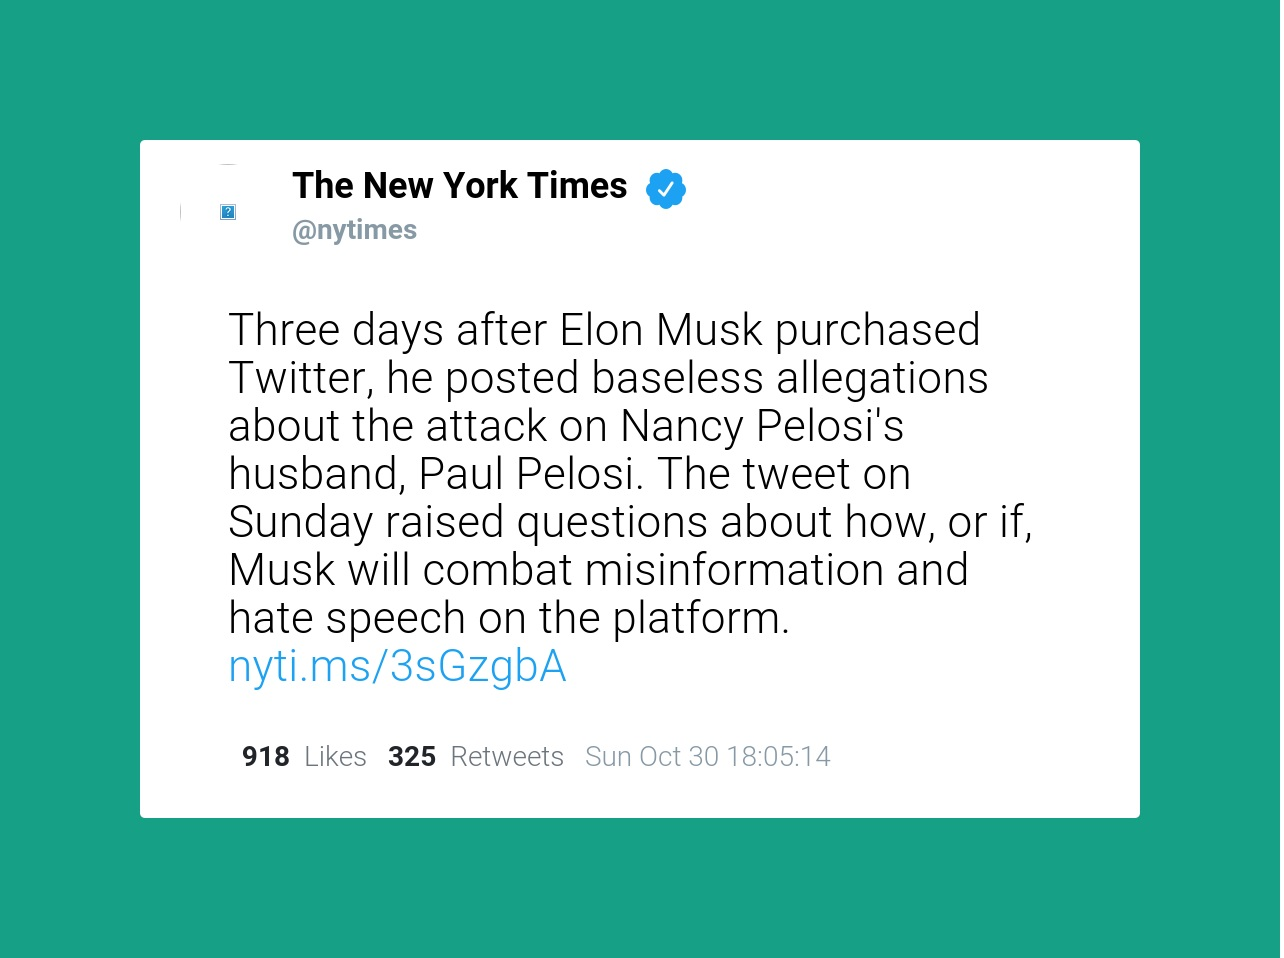
\includegraphics[keepaspectratio]{\%7B\%7Bsite.url\%7D\%7D/img/nyt-musk-misinformation.jpeg}}
\caption{A tweet from the \emph{New York Times} about Elon Musk spewing
misinformation}
\end{figure}

Okay, I am a wee bit worried now. The new CEO to Twitter is essentially
running the site down by posting his own garbage. Who can challenge it?
Frankly nobody. The only way to challenge is to simply walk away at this
point. I'm already in step with
\href{https://twitter.com/popehat/status/1586444996189728768}{``Popehat''
in terms of taking action}.

\begin{figure}
\centering
\pandocbounded{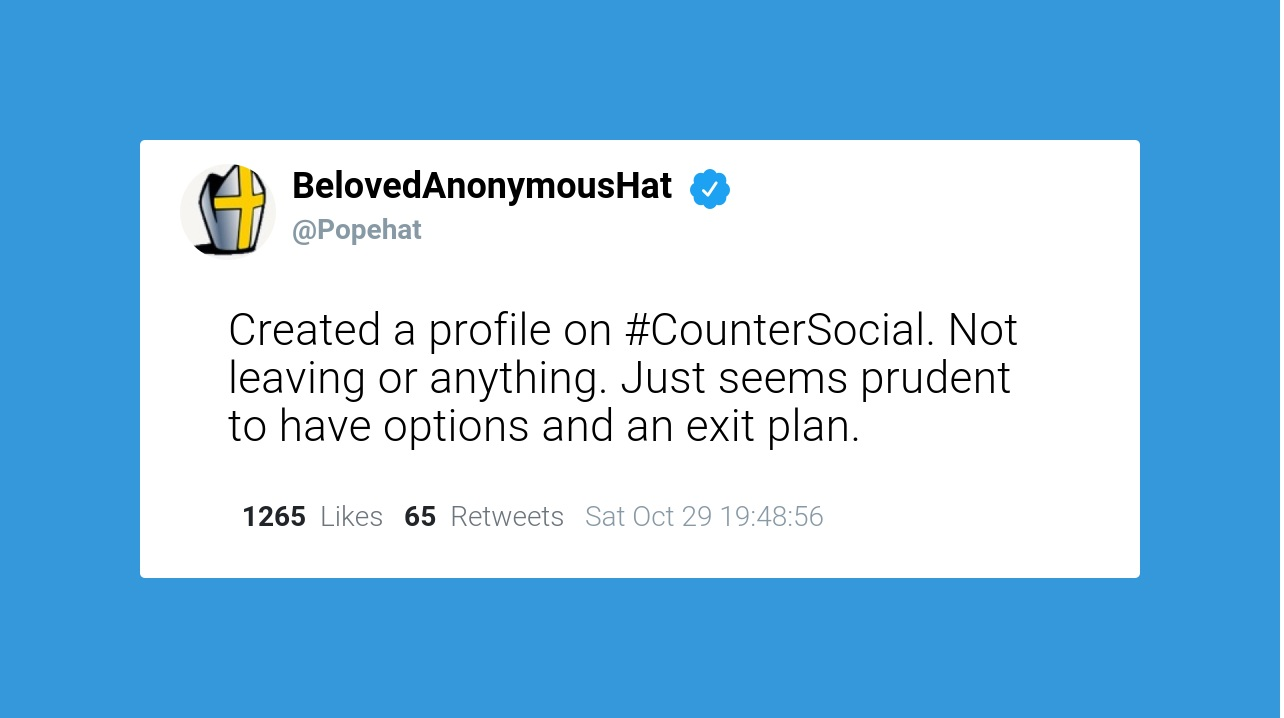
\includegraphics[keepaspectratio]{\%7B\%7Bsite.url\%7D\%7D/img/popehat-create-countersocial-account.jpeg}}
\caption{A tweet from ``Popehat'' stating that he is creating an account
off-Twitter to jump to}
\end{figure}

\href{https://twitter.com/ronfilipkowski/status/1586754844043485191}{Ron
Filipkowski put it sharply}:

\begin{figure}
\centering
\pandocbounded{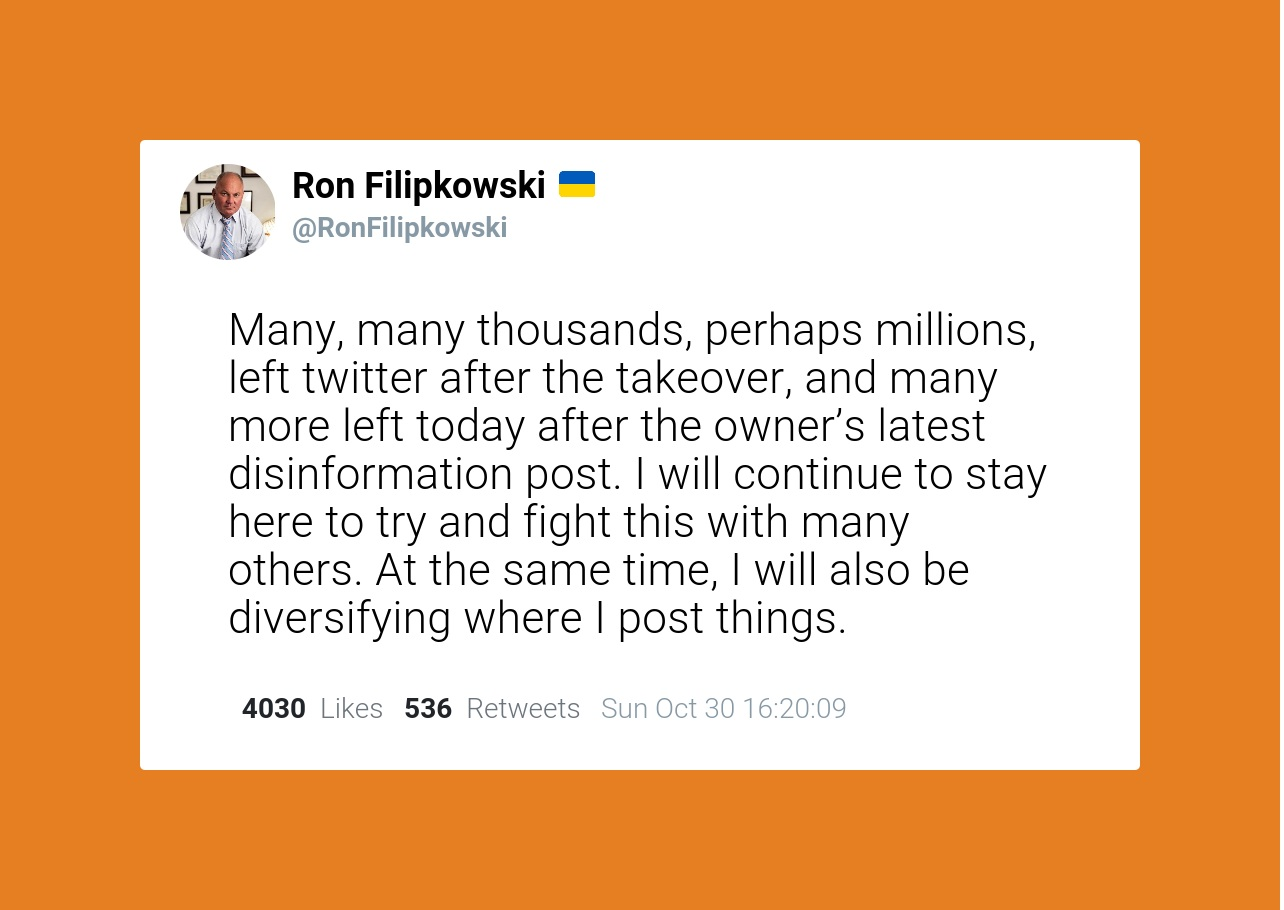
\includegraphics[keepaspectratio]{\%7B\%7Bsite.url\%7D\%7D/img/ronfilipkowski-abandon-ship.jpeg}}
\caption{Ron Filipkowski stating that he is diversifying his online
posting locations}
\end{figure}

Things are just very messy at the moment. We have crazy people attacking
politicians and their families in violation of
\href{https://www.law.cornell.edu/uscode/text/18/351}{the assassination
statue 18 USC 351}. Republicans of the majority faction of the party are
all in a snit trying to secure the levers of power at the moment. The
minority faction is finding itself adrift without a real political home.

There is
\href{https://www.opb.org/article/2022/10/29/ahead-of-election-day-us-agencies-warn-of-potential-attacks-by-extremists/}{already
a joint intelligence bulleting warning of domestic extremism} while
\href{https://www.msn.com/en-us/news/politics/steve-bannon-calls-maga-community-to-arms-says-theyre-the-cavalry/ar-AA13w2Wj}{Steve
Bannon is apparently calling for violence}. POLITICO is
\href{https://www.politico.com/news/magazine/2022/10/29/political-violence-1850s-paul-pelosi-00064107}{drawing
parallels to the 1850s} as to our currently unsettled environment.

If I could accurately predict where things will go then I wouldn't need
to have a day job. I normally have runs of bad luck when visiting
casinos. Preparedness is going to be the key to our near-term weirdness
in America, it seems.

In other news:

\begin{itemize}
\tightlist
\item
  We got the livestream feed fixed so that it will show in the nursery
  in the building. That way anybody who has to head back there can keep
  up with service and not miss out.
\item
  Plans are continuing to be developed for
  \href{https://www.niddk.nih.gov/bwp}{the big project}.
\item
  Eventually I will be doing some radio ``data modes'' stuff on
  shortwave before the end of 2022. It seems prudent.\\
\item
  The project for
  \href{https://code.launchpad.net/~skellat/+git/auto-newspaper}{building
  low-budget community penny press newspapers using LaTeX} will
  hopefully get more attention from me soon.
\end{itemize}
